\documentclass[angelino.tex]{subfiles} 

\begin{document}

This chapter presents the design and implementation
of a practical parallel system for predictive prefetching.
For concreteness, we focus on Metropolis--Hastings in
the case of large-scale Bayesian inference.
%and utilize the estimator we derived in Section~\ref{sec:estimator}
First, we give an overview of our system architecture, which follows a
master-worker pattern.
The master and workers communicate via message passing.
The master keeps track of the state of computational work that could be
performed, is currently in progress or has been completed by the workers.
Importantly, this includes, in the form of probabilities, predictive information
about what work is believed to be the most useful.
The master uses this information to schedule computational work to be completed
by the workers.
In the following section, we describe how the master uses the jobtree,
introduced in Section~\ref{sec:jobtree}, as the central data structure for
managing this information.
Then, we describe our model of execution as it is driven by the messages passed
between the workers and the master.
In the next sections, we provide details about how the master manages
pseudo-randomness and how the workers generate MH proposals.
Finally, we describe our plug-in interface for specifying an instantiation of
MH within our predictive prefetching implementation.


\section{Architectural overview}
\label{sec:architecture}
%  ** Single master, multiple workers \\
%  ** Master maintains probabilities, assigns workers to most probable strings \\
%  ** Workers proceed asynchronously to reduce wait time \\
%  ** Workers abandon work on unproductive areas of the tree \\

Our system architecture follows a master-worker pattern requiring~${J \ge 2}$ parallel cores.
%
One is designated the master and the remaining~${J-1}$ are workers.
%
The main components of our architecture are:
the protocol by which the master and workers communicate,
a data structure for keeping track of computations and their expected utilities,
a scheduler that determines what computational work should be performed by each executor,
and executors that generate proposals and evaluate the target or approximate posteriors.
%
For clarity, we describe our system~\todo{Name?} in the context of Bayesian posterior sampling.
%
Given a target posterior~$\pi(\theta \given \x)$,
proposal distribution~$q(\theta' \given \theta)$,
initial state~$\theta_0$ and number of iterations~$T$,
our system executes a Metropolis--Hastings simulation.
%
The output sequence of samples~${\theta_1, \dots, \theta_T}$ 
is invariant to the number of worker cores.
%
Before describing each architectural component in further detail, we use two
state machines to describe the high-level actions of the master and a worker.
%
We also highlight our use of lazy evaluation principles that make our
implementation practical.

%Before describing each architectural component in further detail, we first give
%a high-level overview of these interacting components.
%%
%The master node maintains a representation of the jobtree and distributes a
%different node in the jobtree to each worker.
%%
%The worker given node~$\rho$ computes the corresponding proposal~$\theta_\rho$
%(which may consume values from the random sequence).
%%
%It asynchronously transmits the proposal, and the new point in the random
%sequence, back to the master.
%%
%It then starts evaluating the target density, producing progressively improved
%approximations to the target that it periodically reports back to the master.
%%
%Meanwhile, the master uses estimates
%of~${{\mcL}(\theta'_\rho) - \mcL(\theta_\rho)}$~\todo{Explain.} values,
%the appropriate~$r_\rho$ constants, and an adaptive estimate of the current
%acceptance probability to calculate the predictor~$\PredEst{\rho}{m}$ for each
%node in the evaluation tree.
%%
%The master assigns workers to execute the target function only for those nodes
%most likely to be on the true path.
%%
%As estimates improve, some workers’ proposals become less likely.
%%
%Workers abandon unlikely proposals in favor of more likely ones.
%%
%If the abandoned proposal becomes likely again, a worker will pick it up where
%the earlier worker left off.


\subsection{Master state machine}
\label{sec:master}

\begin{figure}
\centering
\resizebox{\columnwidth}{!}{
\begin{tikzpicture}[->,>=stealth',shorten >=1pt,auto,node distance=6cm,
                    semithick, line width=1.2pt]
  \tikzstyle{every state}=[fill=LightSteelBlue,draw=none,minimum size=2cm]

  \node[initial,state] (wait)                                      {\wait};
  \node[state]         (schedule)     [above right of=wait]        {\schedule};
  \node[state]         (setproposal)  [below right of=schedule]    {\setproposal};
  \node[state]         (abandon)      [below right of=wait]        {\sendabandon};
  \node[state]         (update)       [below right of=setproposal] {\update};
  \node[state]         (deleteloser)  [below right of=abandon]  {\deleteloser};
  \node[state]         (emit)         [below left of=deleteloser]           {\emit};

  \path (wait)     edge [bend left=10]    node {Receive \WANTWORK} (schedule)
                   edge [bend left=10]    node {Receive \SETPROPOSAL} (setproposal)
                   edge [bend right=10]   node {Receive \UPDATE} (update)
        (setproposal) edge [bend left=10] node {} (wait)
        (schedule) edge [bend left=10]    node {} (wait)
        (update)   edge [sloped, below, bend left=65]  node {Node utility above threshold} (wait)
                   edge [bend left=10]    node {Node complete} (deleteloser)
                   edge [bend left=10]    node {Node utility below threshold} (abandon)
        (deleteloser) edge [bend left=10] node {Node is root's child} (emit)
                      edge [sloped, below, bend left=50] node {Node not root's child} (wait)
        (emit)     edge [bend left=30]    node {} (wait)
        (abandon)  edge [bend left=10]    node {} (wait);
\end{tikzpicture}
}
\vspace{5mm}
\caption{State machine for the master.}
\label{fig:master}
\end{figure}

The central roles of the master are to implement the scheduler that assigns
computational work to each worker, cache the workers' computational results
and emit the simulated Markov chain.
%
The Markov chain starts in some given initial state.
%
We can describe the actions of the master via a state machine,
depicted in Figure~\ref{fig:master}.
%
The master starts in the \wait state, where it waits for any message
from any worker.
%
Eventually, the master receives one of three messages,
\WANTWORK, \SETPROPOSAL or \UPDATE, from a particular worker.
%
Upon receipt of a \WANTWORK message, the master moves to the \schedule state.
There, it identifies useful computational work, replies to the worker
with a \HAVEWORK message and returns to the \wait state.
%
Upon receipt of a \SETPROPOSAL message, the master moves to the \setproposal state.
The \SETPROPOSAL message contains a proposal computed by the worker,
which the master caches before returning to the \wait state.
%
Upon receipt of an \UPDATE message, the master moves to the \update state.
The \UPDATE message contains information that improves the predictor for some
node~$\rho$ in the jobtree, as described in Section~\ref{sec:predictive-prefetching}.
The master uses this information to update the predictor~$\Predictor{\rho}$.

Once the master applies the last update at a node, the node becomes \emph{complete}.
If both~$\rho$ and~$\rho$'s comparison parent are complete, then the predictor~$\Predictor{\rho}$
converges to the indicator in Equation~\ref{eqn:indicator}.
In this case, one of~$\rho$'s children has branch probability~$1$
and the other has branch probability~$0$.
Consequently, this latter child's entire subtree has utility~$0$.
The master moves to the \deleteloser state, where it deletes this subtree.
If~$\rho$ is complete but is not the child of the root in the jobtree,
then the master returns to the \wait state.
Otherwise, the master now knows the result at the immediate transition
and moves to the \emit state.
There, the master emits one or more of the next states of the Markov chain.
The master also integrates garbage collection with updating,
and at this point trims portions of the jobtree that are no longer relevant.
This could alternately have been integrated with the master's response to
some other periodic worker message.
Either way, there is no separate garbage collection `process.'
From the \emit state, the master returns to the \wait state.

If the update does not contain enough information for the predictor to
converge to the indicator, the master may optionally reconsider whether
further computation at node~$\rho$ is still of interest.
If the master decides that the expected utility of~$\rho$ is above some
threshold, then it returns back to the \wait state; in this case, the worker
continues work on the current node.
Otherwise, the master moves to the \sendabandon state, where it sends the
worker an \ABANDON message, telling the worker to stop its current computation.
From the \sendabandon state, the master returns to the \wait state.

\subsection{Worker state machine}
\label{sec:worker}

The central role of a worker is to implement an executor that performs
computational work scheduled by the master.
%
We depict the state machine of a worker in Figure~\ref{fig:worker}.
%
The worker starts in the \want state, in which it sends the master a \WANTWORK
message indicating that it is ready for a new assignment of computational work.
%
The worker leaves the \want state once it receives a \HAVEWORK message from the
master containing such an assignment.


\begin{figure}[t!]
\centering
\resizebox{\columnwidth}{!}{
\begin{tikzpicture}[->,>=stealth',shorten >=1pt,auto,node distance=7cm,
                    semithick, line width=1.2pt]
  \tikzstyle{every state}=[fill=LightSteelBlue,draw=none,minimum size=2cm]

  \node[initial,state] (want)                             {\want};
  \node[state]         (init)       [above right of=want]       {\init};
  \node[state]         (continue)   [below right of=init] {\continue};
  %\node[state]         (update)     [below left of=continue]    {\sendupdate};
  \node[state]         (check)      [below right of=want]  {\check};

  \path (want)     edge [bend left]      node {Receive \HAVEWORK w/o proposal} (init)
                   edge [bend left=40]  node {Receive partial \HAVEWORK} (continue)
        (init)     edge [bend left]      node {} (continue)
        (continue) edge [above, bend right=10]      node {Complete last quantum} (want)
                   edge [bend left]   node {Complete quantum} (check)
        %(continue) edge [bend left]            node {} (update)
        %(update)   edge [bend left]            node {} (check)
        (check)    edge [bend left]      node {\ABANDON received} (want)
        edge [bend left]             node {No \ABANDON received} (continue);
\end{tikzpicture}
}
\vspace{5mm}
\caption{State machine for a worker.}
\label{fig:worker}
\end{figure}

If the worker receives a \HAVEWORK message for a node~$\rho$ in the jobtree 
such that the message does not contain the state~$\theta_\rho$,
then the worker moves to the \init state.
%
Note that the first \HAVEWORK message for the root of the jobtree contains the
initial state~$\theta_0$, while the first \HAVEWORK message for any other node
does not contain the corresponding state, which in this latter case is always a
proposal.
%
In the \init state, the worker generates the proposal~$\theta_\rho$ at node~$\rho$
and can compute functions of~$\theta_\rho$, \eg in Bayesian posterior sampling,
the prior~$\pi_0(\theta_\rho)$ in Equation~\ref{eq:poserior} is only a function 
of~$\theta_\rho$.
%
The worker sends these results to the master and then moves to the \continue state.
%
The worker could alternately receive a work assignment to resume computation at
a partially evaluated node; in this case, it moves directly from the \want state to
the \continue state.

In the \continue state, the worker performs computation that contributes to
forming a predictor~$\Predictor{\rho}$ for the given node~$\rho$.
%
For example, it may compute a fast approximation to the target likelihood evaluated
at~$\theta_\rho$, which together with the prior produces an approximate posterior.
%
Alternatively, it may complete the exact target evaluation of interest,
or any incremental portion of any approximate target or the exact target.
%
After computing some \emph{quantum}, \ie useful unit of computation,
the worker moves to the \sendupdate state, where it sends a message to the
master containing the latest results produced while in the \continue state.
%
If at this point the worker has completed the last assigned quantum at
node~$\rho$, then it moves back to the \want state.
%
Otherwise, the worker enters the \check state, where it checks whether it has
received an \ABANDON message from the master instructing it to stop its current
computation.
%
If it has received such a message, then it returns to the \want state;
otherwise, it returns to the \continue state.

\subsection{Practical considerations}
\label{sec:practical}

Lazy evaluation is an important principle that makes our implementation practical.
%
In particular, our central data structure is a binary tree with depth equal
to the number of desired Metropolis--Hastings samples,
\ie the number of iterations in the equivalent serial execution;
in our empirical studies designed to be representative of realistic scenarios,
this number is 50000.
%
We only materialize small portions of the tree as they become useful for
prefetching; we never materialize the whole tree.
%
Furthermore, the expected utilities change as computations are updated and
completed, so we lazily compute expected utilities only as they are needed,
instead of continuously updating them.

%%%%%%%%%%%%%%%%%%%%

\section{The jobtree}
\label{sec:the-jobtree}

Central to our architecture is a data structure for
keeping track of computations and other information relevant to managing a
MCMC simulation within the predictive prefetching framework.
%
This data structure is used for caching the results of computation performed by
the workers, including speculative and partial computation.
%
Furthermore, it must be able to maintain and update probabilistic beliefs about
the utilities of different computations that have been or could be performed
or are currently in progress.
%
During the course of execution, this data structure must reflect when
these beliefs eventually converge to certainty and thus support the construction
of output exactly equal to the equivalent serial computation.
%
Importantly, it must be efficient to query this data structure for computational
work that is not complete, is not currently being performed by any worker
and is believed to be significantly useful.
%

A tree supports our data structure requirements.
%
Specifically, the master maintains a representation of the jobtree,
introduced in Section~\ref{sec:jobtree}.
%
Every node~$\rho$ in the jobtree is associated with %a bit string~$\rho$,
a state~$\theta_\rho$ and full, partial or approximate computation of the target
density at that state.
If the full target density~$\pi(\theta_\rho \given \x)$ has been computed,
then we mark the node as \emph{complete}; otherwise, the partial or approximate
computation provides an estimate~$\tilde\pi(\theta_\rho \given \x)$
and we mark the node as \emph{incomplete}.
%
Every node~$\rho$, except the root, has a right child~$\rho\bits{1}$,
a left child~$\bitsflip{\rho}\bits{1}$ and
a comparison parent~$\truncbits{\bitsflip{\rho}}$.
The root~$\emptystr$ has a single (right) child~$\emptystr\bits{1}$.
%
Every node~$\rho$, except for the root, is a proposal and
has a predictor~$\Predictor{\rho}$ equal to the conditional probability
that~$\theta_\rho$ is accepted, given that~$\rho$ is on the true computation path.
%
%Recall that if~$\rho$ is accepted, then the next proposal to consider is 
%the right child~$\rho\bits{1}$; otherwise,~$\rho$ is rejected and the next
%proposal to consider is the left child~$\bitsflip{\rho}\bits{1}$. 
%
%If~$\rho$ and~$\rho$'s comparison parent are both complete,
%then~$\Predictor_\rho$ is either exactly~0 or exactly~1;
%otherwise, it is neither exactly~0 nor exactly~1.
%
For convenience, we set the root's predictor to~1.
%
Every node also has an expected utility, \ie probability of being on the
true computation path.
The root's (expected) utility is 1.
For every other node~$\rho$, the expected utility is the product of the branch 
probabilities along the path connecting the root to~$\rho$.
Recall that the branch probabilities label the edges and are related to the
predictors: the edge from a node~$\rho$ to its right child has branch
probability equal to the predictor~$\Predictor{\rho}$ and the edge to its left
child has branch probability~${1 - \Predictor{\rho}}$.

Our jobtree includes several features specific to our implementation.
As described in Section~\ref{sec:practical},
the master lazily computes the expected utility of a node~$\rho$
whenever called for by traversing the path from the root to~$\rho$.
Thus, the expected utilities are not explicitly represented at each node in the jobtree.
%
Also, every node~$\rho$ may have at most one \emph{executor}, \ie the worker
core computing~$\pi(\theta_\rho \given \x)$, and optional executor status
information, such as how much partial computation has been completed so far.
An extension to our implementation would be to have multiple executors per node,
an idea explored by~\citet{strid-2010-prefetching} and by us in
Section~\ref{sec:multi-way},
and that we discuss further in Chapter~\ref{sec:conclusions}.
%
Finally, every node is marked with one of three designations.
A \emph{dead} node has utility~0; it cannot be part of the true computation path. 
A \emph{pending} node is incomplete, has positive expected utility and has no executor.
An \emph{active} node is incomplete, has positive expected utility, and has an executor.


\section{Selecting high-utility pending nodes}
\label{sec:highest-utility-pending}

One of the master's jobs is to assign workers to the pending nodes with highest
utility.
%
In our initial implementation, the master maintained a priority queue
called the \emph{pending queue}.
%
It contained all pending nodes in the tree, ordered by \emph{ascending} expected
utility, \ie the head of the pending queue was the inactive node with the
highest expected utility.

We observed that the pending queue was actually redundant with the jobtree,
as the latter data structure contained all the same information.
%
This suggested an alternative stochastic routine, described next,
that allowed us to eliminate the pending queue.
%
To assign a worker to a node, the master stochastically traverses the
jobtree from the root, following branches according to their branch
probabilities, until it finds a pending node, \ie a node that is neither active
nor dead and has no executor.
%
In this way, the master stochastically assigns workers to those nodes with
highest expected utility.

\section{Execution and messaging protocol}
\label{sec:execution}

Our system's execution is driven by the messages communicated from the workers
to the master and vice versa.
%
The protocol by which they communicate is implicit in their state machines,
described in Section~\ref{sec:architecture}.
%
We present our model of execution and messaging protocol together
by considering the various possible scenarios that may occur.

%Figure~\ref{fig:protocol} summarizes the messaging protocol.
%
%\begin{figure}[h]
%\centering
%\includegraphics[width=0.49\textwidth]{figs/protocol.pdf}
%\caption{Summary of the protocol by which the master and workers communicate.}
%\label{fig:protocol}
%\end{figure}

Initially, the jobtree contains two nodes,~$\emptystr$ and~$\bits{1}$.
%
Both of these nodes have (expected) utility~1.
%
The predictor~$\Predictor{\bits{1}}$ is initialized to~0.5, reflecting that we
initially have no information about whether the first proposal will be accepted
or rejected.
%
The master can send or receive messages to any worker
and each worker can send or receive messages to the master;
the workers do not communicate with each other.
%
From the master's state diagram in Figure~\ref{fig:master}, we can see that its
actions are responsive, \ie it starts in the \wait state, leaves only to
respond to a message from a worker, and always returns to the \wait state.


\begin{figure}[t]
\centering
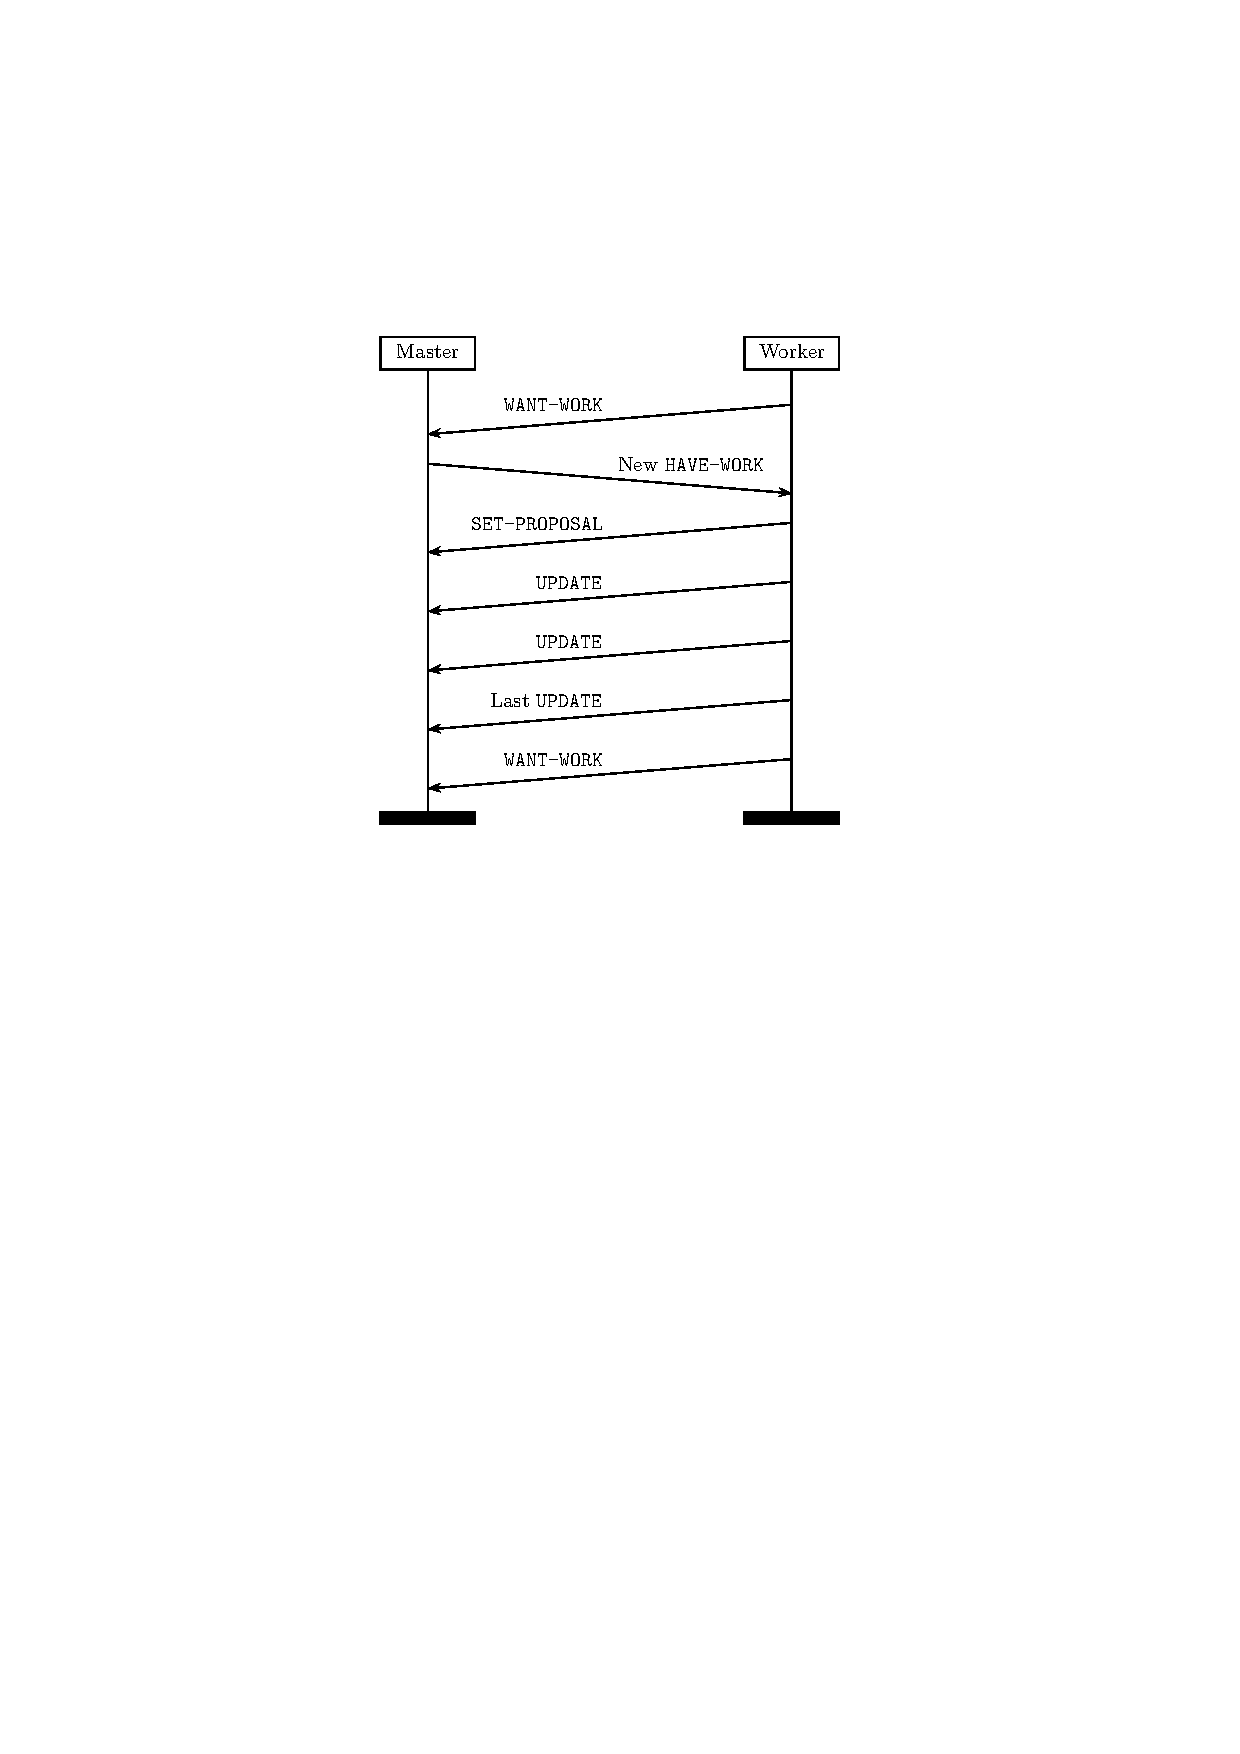
\includegraphics[width=0.49\textwidth]{figs/protocol/new-work.pdf}
\caption{Simplest scenario in which a worker asks for work via a \WANTWORK
message and receives a new \HAVEWORK message for a particular node in the jobtree.
The worker performs all the work at this node, sending partial results along the way.
The proposal, and potentially, initial computational results involving the proposal,
are contained in a single \SETPROPOSAL message.
Subsequent computational results are contained in one or more \UPDATE messages.
When the worker is finished, it requests new work with via another \WANTWORK message.
For simplicity, this diagram contains only one worker.}
\label{fig:new-work}
\end{figure}

Workers initiate execution by requesting work from the master via a
\WANTWORK message.  This is the first action of each worker.
%
We summarize the simplest initial series of messages, starting with such a
\WANTWORK message, in Figure~\ref{fig:new-work}.
%
When the master receives a \WANTWORK message from worker~$W$,
it finds a pending node with high expected utility, as described in 
Section~\ref{sec:highest-utility-pending}.
%
The master replies to worker~$W$ with a \HAVEWORK message
containing~$\rho$ and, if known, the state~$\theta_\rho$, and otherwise,
it also contains whatever information is available to generate~$\theta_\rho$
most efficiently.
%
Precisely what information this is will become clear in
Sections~\ref{sec:handling-randomness} and~\ref{sec:gen-proposals};
for now, note that~$\theta_\rho$ can be generated from its comparison
parent,~$\theta_{\truncbits{\bitsflip{\rho}}}$, given the appropriate
position in the pseudorandom stream.
Further, recall that the log (unnormalized) target posterior decomposes as
\be
{\mcL}(\theta_\rho) = \log \pi(\theta \given \x) =
\log \pi_0(\theta) + \sum_{n=0}^{N-1} \log\pi(x_n \given \theta).
\label{eq:metric-sum}
\ee
In our implementation, workers compute the above sum of likelihood terms 
in batches of size~$b$, and thus it may have already been partially evaluated.
Also in batches, workers compute the sum of squared likelihood terms
\be
\sum_{n=0}^{N-1} (\log\pi(x_n \given \theta))^2
\label{eq:metric-sum-squares}
\ee
used by the master to estimate the error in using a partially
evaluated target to approximate the true target.	
Thus, the \HAVEWORK message also includes the results of having partially
evaluated Equations~\ref{eq:metric-sum} and~\ref{eq:metric-sum-squares},	
as well as an index~$m$, where ${0 \le m < N-1}$ and~${m \mod b = 0}$,
indicating where the worker should resume computation.
%
The master then marks~$\rho$ as active and sets~$\rho$'s executor to~$W$.
%
If $\rho$ does not yet have any children in the jobtree, the
master also creates $\rho$'s children, each of which it marks as pending.
For each new node~$\phi$, its predictor~$\Predictor{\phi}$ 
is initialized to the \emph{local acceptance rate}, which we define to be
empirical acceptance rate observed during simulation of the~$k$ most
recent Metropolis--Hastings samples.
In our implementation,~${k = \min\{t, 100\}}$, where~$t$ is total number of
MH~samples obtained thus far.


A \HAVEWORK message for node~$\rho$ contains the partially evaluated target
posterior in Equation~\ref{eq:metric-sum}, the partially evaluated sum of
squared likelihood terms in Equation~\ref{eq:metric-sum-squares}, an index~$m$
and, if~$m > 0$, the state~$\theta_\rho$.
%
Figure~\ref{fig:new-work} depicts the scenario where the \HAVEWORK message does
not contain~$\theta_\rho$.~\todo{Add letters to Fig.}
In this case, the worker first generates~$\theta_\rho$,
as described in Section~\ref{sec:gen-proposals},
and then computes the log prior~$\log\pi_0(\theta_\rho)$.
The worker replies to the master with a \SETPROPOSAL message
containing~${\rho, \theta_\rho}$ and~$\log\pi_0(\theta_\rho)$.
The master stores the information from this message in the jobtree, \ie it 
stores~$\theta_\rho$ and, if relevant,~$\log \pi_0(\theta_\rho)$ at node~$\rho$.

\begin{figure}[t]
\centering
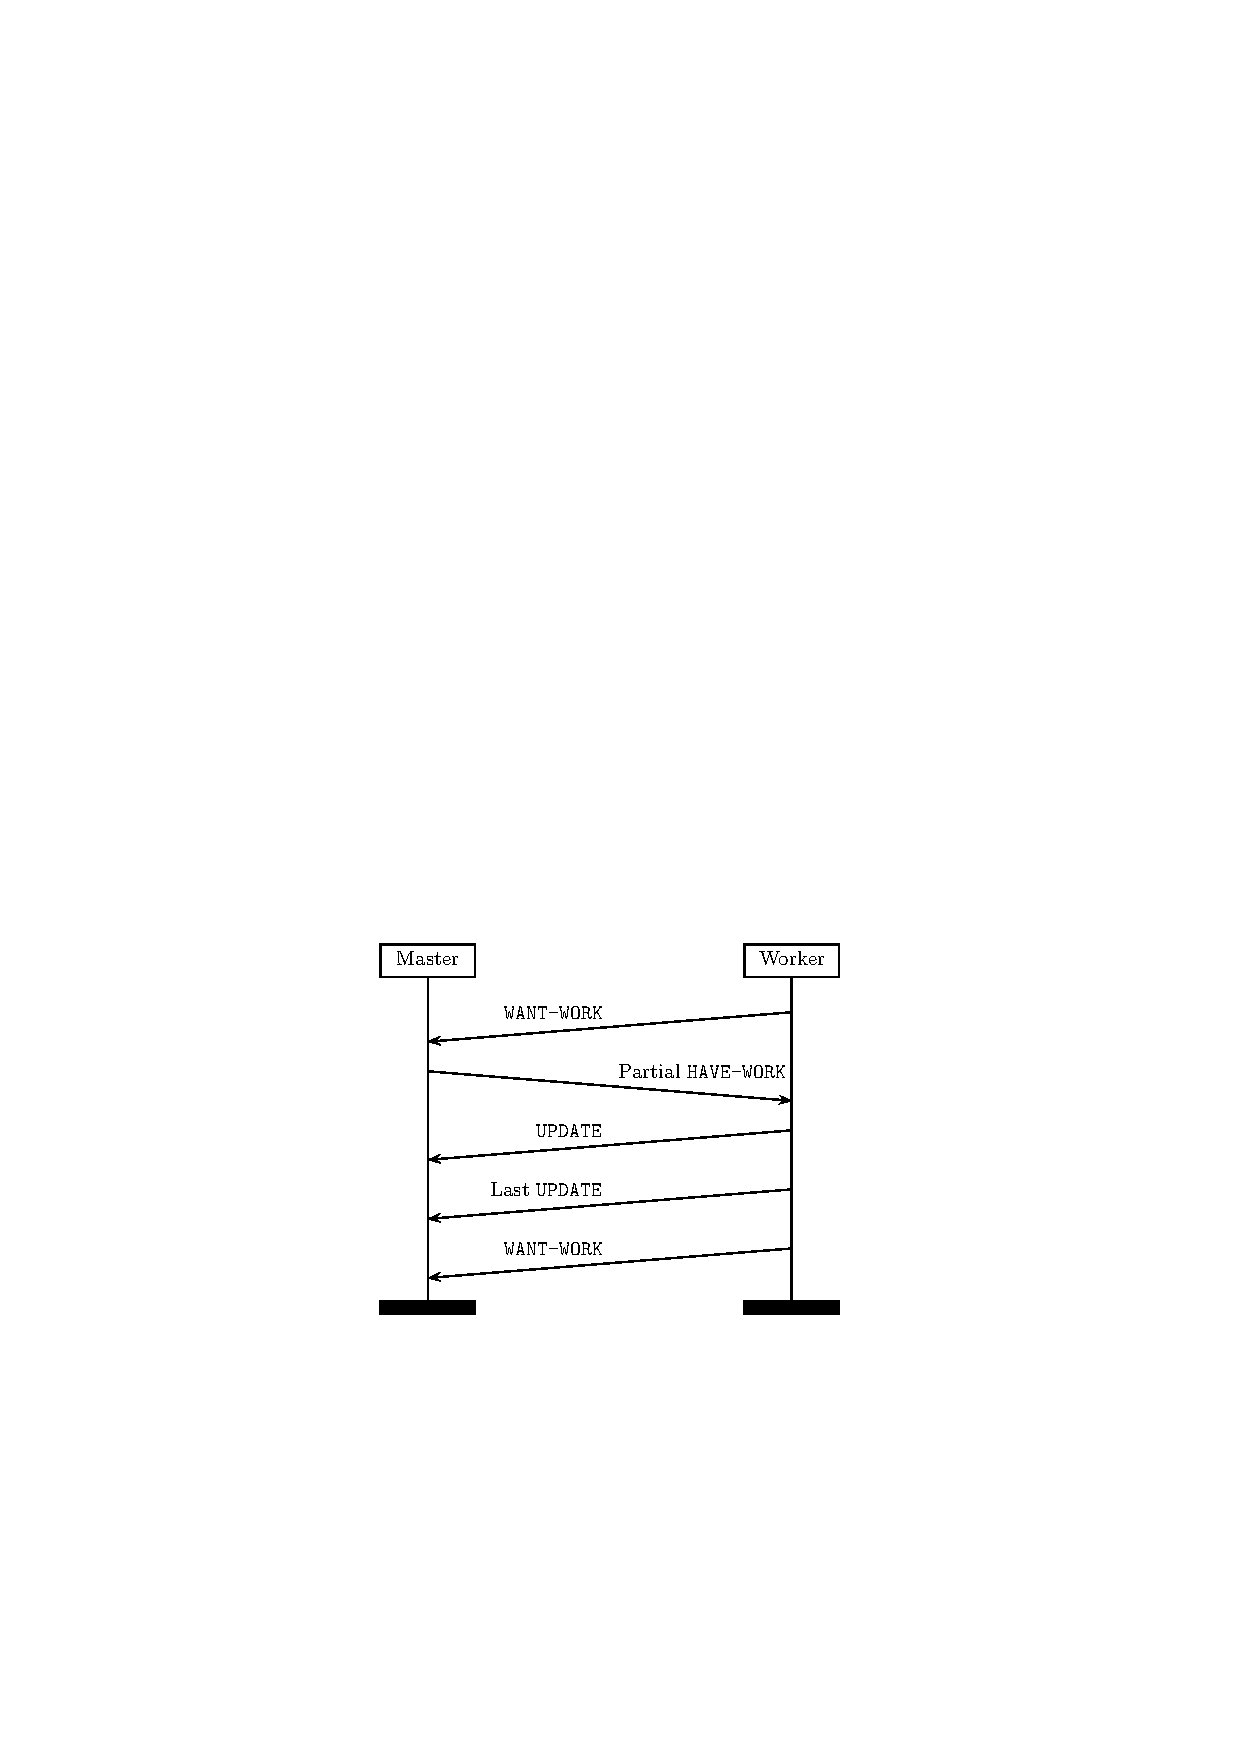
\includegraphics[width=0.49\textwidth]{figs/protocol/partial-work.pdf}
\caption{Scenario in which a worker receives a partial \HAVEWORK message
for node~$\rho$ that already contains the state~$\theta_\rho$,
and potentially, additional partial results.}
\label{fig:partial-work}
\end{figure}

Alternately, the \HAVEWORK message already contains the proposal,
and potentially, additional partial results; this scenario is depicted in Figure~\ref{fig:partial-work}.
%
In either case, the worker proceeds with computing the target posterior in 
Equation~\ref{eq:metric-sum} and sum of squared likelihood terms in 
Equation~\ref{eq:metric-sum-squares}, in batches of size~$b$ starting at index~$m$.
%	
After each completed batch, the worker sends an \UPDATE message to the
master containing the updated values of the partially evaluated
target posterior and sum of squared likelihood terms,
as well as an index~$m' > m$, indicating how far these
incremental computations have progressed in total.
%
The worker periodically checks for any \ABANDON messages from the
master.
Upon receiving such a message, the worker discontinues work on
node~$\rho$ and sends the master a \WANTWORK message.
We depict this scenario in Figure~\ref{fig:abandon}.
In our implementation, the worker makes these checks after each completed batch.
%
After the worker sends the last \UPDATE message for the last batch,
it sends the master a \WANTWORK message.


\begin{figure}[t]
\centering
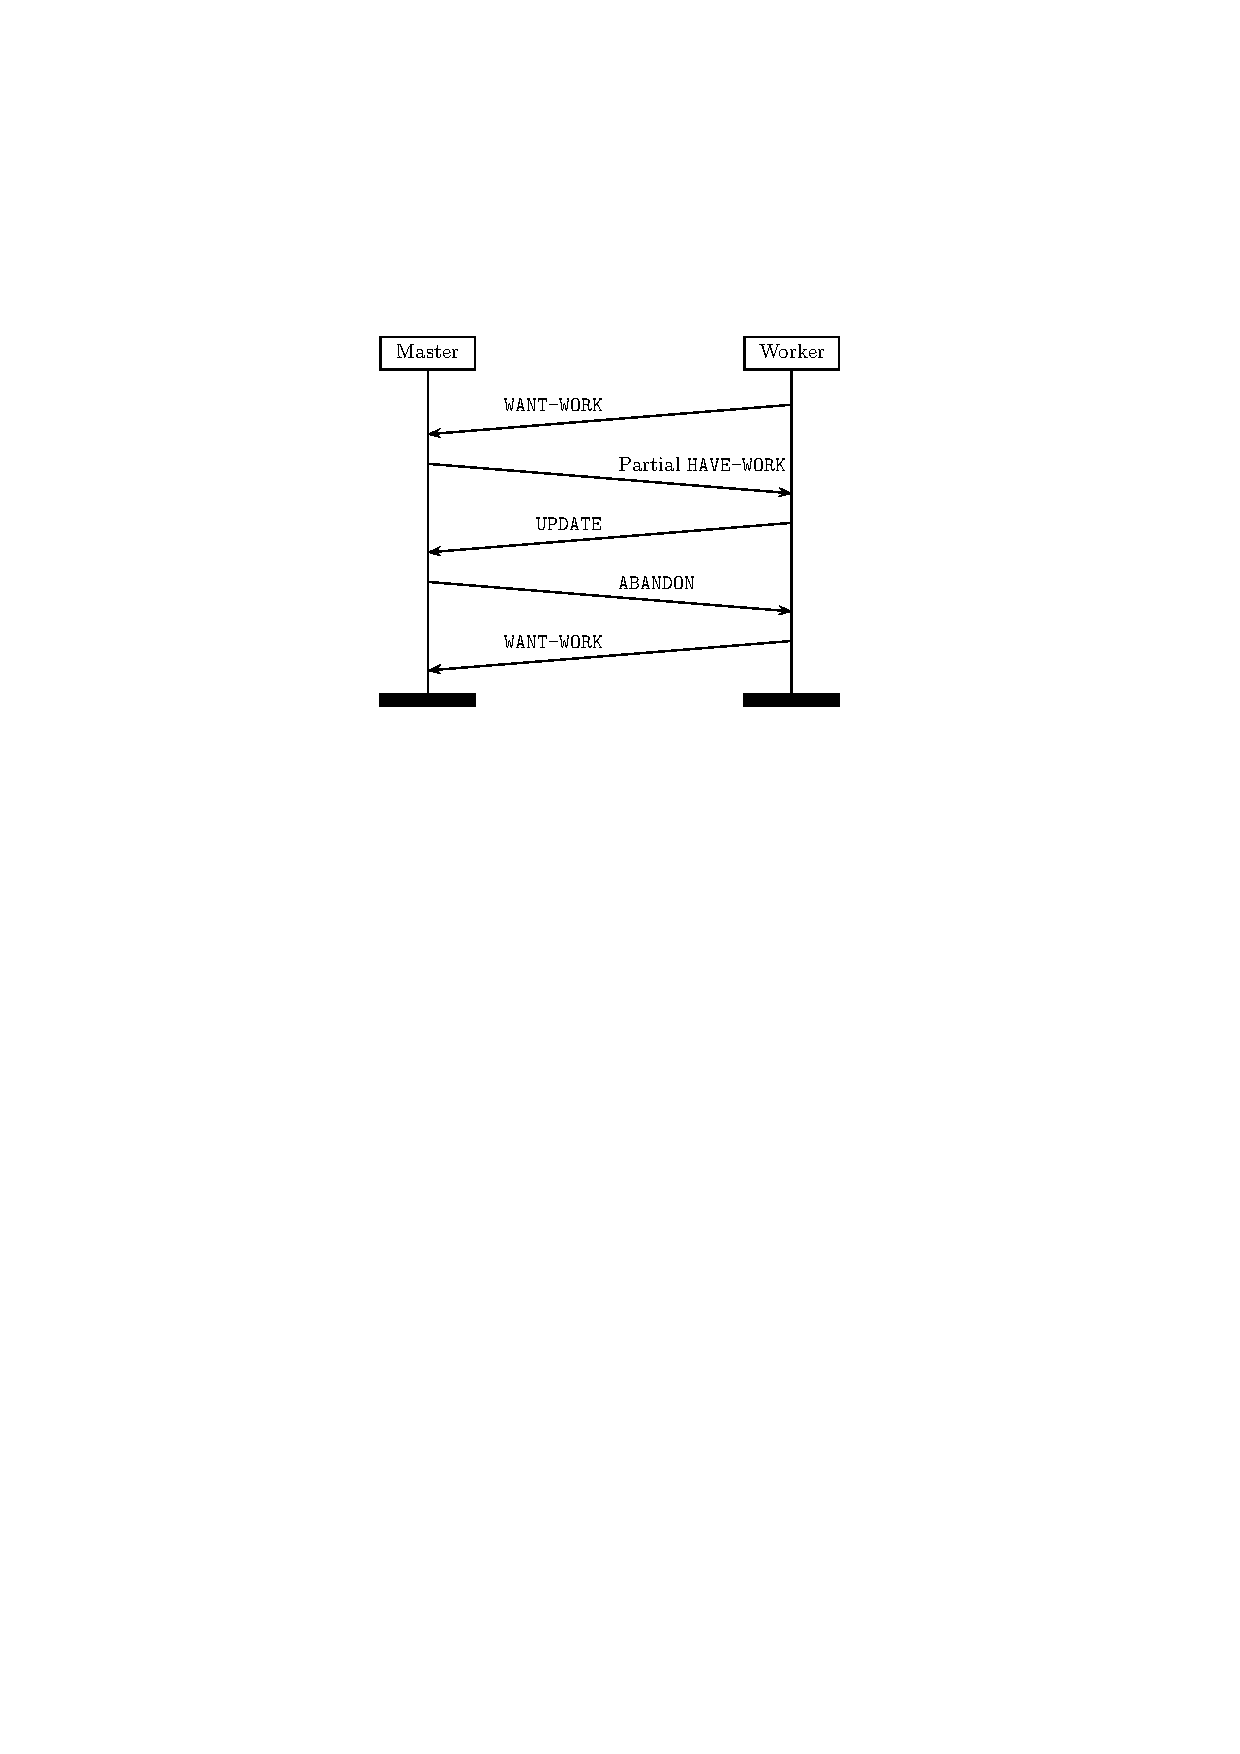
\includegraphics[width=0.49\textwidth]{figs/protocol/new-work-abandon.pdf}
\caption{Scenario in which a worker receives an \ABANDON message.
If an \UPDATE from a worker results in the expected utility of the node dropping
below some threshold, then the master sends an \ABANDON message.}
\label{fig:abandon}
\end{figure}


Now suppose the master receives an \UPDATE message for node~$\rho$ from a worker;
we depict such messages in Figures~\ref{fig:new-work},~\ref{fig:partial-work}
and~\ref{fig:abandon}.
%
At node~$\rho$ in the jobtree, the master updates its estimate of the log
posterior as in Equation~\ref{eq:metric-sum} and the error of this estimate
as in Equation~\ref{eq:metric-sum-squares}.
%
Next, the master updates the branch probabilities, introduced in 
Section~\ref{sec:predictive-prefetching},
of node~$\rho$ and any nodes for which~$\rho$ is the comparison parent.
%
Recall that each Metropolis--Hastings transition stochastically chooses between
two states -- where one is the comparison parent of the other -- by comparing
their posterior evaluations relative to a uniform random variate.
%
Consider one of these branch probability updates, such that~$\rho$ is the
comparison parent of a node corresponding to the proposal~$\theta'_\rho$
with uniform variate~$u$.
%
Recall from Section~\ref{sec:predictive-prefetching} that 
the edge from a node~$\rho$ to its right child has branch probability equal to
the predictor~$\Predictor{\rho}$ and the edge to its left child has
branch probability~${1 - \Predictor{\rho}}$.
%
To update the predictor~$\Predictor{\rho}$ in Equation~\ref{eqn:subset},
the master computes an estimate of the difference of log posteriors as in
Equation~\ref{eqn:difference},
\[
{\mcL}(\theta_\rho) - {\mcL}(\theta_\phi) =
\log \pi(\x \given \theta_\rho) - \log \pi(\x \given \theta_\phi),
\]
the error of this estimate corresponding to Equation~\ref{eqn:sigma}
and the constant value
\[
r = u \frac{q(\theta'_\rho \given \theta_\rho)}{q(\theta_\rho \given \theta'_\rho)}.
\]
We elaborate on the details of this calculation in Section~\ref{sec:predictor-implementation}.
In all of our experiments, the proposal distribution~$q(\cdot \given \cdot)$ is
symmetric, in which case~$r = u$.

When the master applies the last update at node~$\rho$, the node becomes complete.
If both~$\rho$ and~$\rho$'s comparison parent are complete,
then the predictor~$\Predictor{\rho}$ converges to the indicator in
Equation~\ref{eqn:indicator} and the master deletes the subtree with utility~$0$.
If~$\rho$ is the child of the root in the jobtree,
\ie the immediate transition chooses between the states at these two nodes,
then the master emits the next state of the Markov chain, which is now
completely specified, and also emits any subsequent states of the Markov chain
whose predictors have already converged to the indicator.
Each time the next state of the Markov chain is emitted,
the root of the jobtree is removed and the emitted state becomes the new root.
If the emitted state corresponds to an accepted proposal,
the root's (only) child becomes the new root and the left subtree is trimmed away.
Otherwise, the proposal was rejected and old root is still the new root,
but needs to be connected to the left subtree at its left grandchild
(with bit string~$\bits{01}$) and the right subtree is trimmed away.

If the update does not contain enough information for the predictor to converge
to the indicator, the scheduler may optionally reconsider whether further
computation at node~$\rho$ is still of interest.
Recall that each updated branch probability may change the expected utilities
of descendant nodes that are pending.
The master lazily updates the expected utility of~$\rho$ and identifies a
high-utility pending node~$\phi$ following the procedures outlined in
Sections~\ref{sec:practical} and~\ref{sec:highest-utility-pending}.
If the expected utility of~$\phi$ is significantly
greater than that of~$\rho$, the master marks~$\rho$ as pending and
sends the worker an \ABANDON message, depicted in Figure~\ref{fig:abandon}.
%
Note that any partial computations at an abandoned node remain cached on the
jobtree until the node is trimmed.
Such abandoned nodes can later be reassigned to workers if their expected
utility increases relative to the active nodes.
Any subsequent workers will resume computation where the previous worker left off.

In all of our experiments, the master decides to abandon~$\rho$ if the
expected utility of~$\phi$ is at least a factor of~$1.1$ greater than that of~$\rho$.
This threshold, which we observed empirically to be effective, balances the
ideal policy -- keeping the workers active at those nodes with highest expected
utility -- with the actual implementation costs of reassigning nodes to workers,
which include some bookkeeping and communication.

%When master receives UPDATE(W, $\alpha$, p, metric): \\
%   // metric is the metric at position p \\
%   Let $\beta$ = the comparison node for $\alpha$ \\
%   Calculate BP($\alpha$) using metricsum($\alpha$) and metricsum($\beta$) and randomnumberchosenfor($\alpha$) \\
%      NB important to use metricsum($\beta$) close to position p \\
%      Maybe something here about uncertainty and approximation \\
%   If evaluation of $\alpha$ is complete, or P($\alpha$) is too small \\
%          (there are N higher-probability strings), then \\
%      send ABANDON \\
%   else \\
%      send OK \\
%
%Suppose worker~$W$ is performing computation associated with node~$\rho$.
%If the master sends~$W$ an \ABANDON message, the master
%first updates $\rho$'s metric, as above.
%%
%Next, it unregisters~$W$ as the executor for~$\rho$.
%%
%If~$\rho$ is not dead, then the master marks~$\rho$ as pending.


\section{Managing pseudo-randomness}
\label{sec:handling-randomness}

Prefetching schemes require careful management of pseudo-randomness to yield
output that is invariant to the number of worker cores, and, as a consequence, 
is exactly equal to an equivalent serial execution.
%
In Section~\ref{sec:using-randomness}, we outlined several strategies for
achieving this.
%
Here, we describe our approach, in which our system synchronizes the use of
pseudo-randomness to our notion of ground truth corresponding to serial execution.

Our implementation follows directly from the mathematical framework
presented in Section~\ref{sec:mathematical-framework}.
%
Recall that progressing from one level to the next in the MH binary tree,
or equivalently the jobtree, corresponds to one application of the MH transition 
operator.
%
For a large class of MCMC algorithms, we showed how to decompose the
transition operator~${T:\X\times\mcU\to\X}$ into two functions.
%
The first function~${Q:\X\times\mcU_Q\to\mcP(\X)}$, produces a countable set of
candidate points in~$\X$, where~$\mcP(\X)$ is the power set of~$\X$.
%
The second function~${R:\mcP(\X)\times\mcU_R\to\X}$ then chooses one of the 
candidates for the next state in the Markov chain.
%
$\mcU_Q$ and~$\mcU_R$ indicate disjoint subspaces of the unit hypercube~$\mcU$
relevant to each part of the operator.
%
%We illustrated this for the special case of Metropolis--Hastings
%in Algorithm~\ref{mh-decomposed},
%reproduced here as Algorithm~\ref{mh-decomposed-repeat}.
%
In Metropolis--Hastings,~$\mcU_Q$ corresponds to the pseudo-random numbers 
consumed to generate proposals and~$\mcU_R$ corresponds to the uniform random
variates used to stochastically accept or reject proposals.


\begin{figure}[t!]
  \centering%
  \resizebox{\columnwidth}{!}{%
    \def\radius {8mm}
    \tikzstyle{state}=[circle, thick, minimum size=\radius, font=\footnotesize, draw]
    \tikzstyle{empty}=[circle, minimum size=\radius, font=\footnotesize]
    \tikzstyle{compute}=[circle, thick, fill=CornflowerBlue, inner sep=0pt, minimum size=\radius, font=\footnotesize, draw]
    \begin{tikzpicture}[->,>=stealth',level/.style={sibling distance = 10cm/#1, level distance = 1.8cm}]
      \draw [gray,-] (-6cm,-1.2cm) -- (6cm,-1.2cm);
      \draw [gray,-] (-6cm,-3.0cm) -- (6cm,-3.0cm);
      \draw [gray,-] (-6cm,-4.8cm) -- (6cm,-4.8cm);
      \node [state] {$x^0_\emptystr$}
      child{ node [state] {$x^1_\bits{1}$} 
        child{ node [state] {$x^2_\bits{01}$}
          child{ node [state] {$x^3_\bits{001}$}
          edge from parent node[left] {$u_Q^4, u_Q^5$} }
          child{ node [state] {$x^3_\bits{011}$}
          edge from parent node[right] {$u_Q^4, u_Q^5~$} }
          edge from parent node[left] {$u_Q^2, u_Q^3~~$} 
        }
        child{ node [state] {$x^2_\bits{11}$}
          child{ node [state] {$x^3_\bits{101}$}
          edge from parent node[left] {$u_Q^6, u_Q^7~$} }
          child{ node [state] {$x^3_\bits{111}$}
          edge from parent node[right] {$u_Q^6, u_Q^7, u_Q^8, u_Q^9$} }
          edge from parent node[right] {$~u_Q^2, u_Q^3, u_Q^4, u_Q^5$}
        }
        edge from parent node[left] {$u_Q^0, u_Q^1$} 
      }
      ;
      \node [empty] at (-5.5cm, -0.9) {$u_R^0$};
      \node [empty] at (-5.5cm, -2.7) {$u_R^1$};
      \node [empty] at (-5.5cm, -4.5) {$u_R^2$};
    \end{tikzpicture}
  }
  \caption{Consumption of pseudo-randomness with respect to the
  Metropolis--Hastings jobtree.
  Edges are labeled by elements from the pseudo-random
  sequence~$\{u_Q^0, u_Q^1, u_Q^2, \dots\}$ consumed during proposal generation.
  Each layer also requires one element of a separate pseudo-random
  sequence~$\{u_R^0, u_R^1, u_R^2, \dots\}$, shown on the left, corresponding to
  the uniform random variate used in the stochastic accept/reject decision.
  In general, each proposal generation may require a variable number of sequence
  elements.
}
  \label{fig:random}
\end{figure}


In our implementation of MH within the prefetching framework, the proposals are
generated on the workers and the decision to accept or reject a proposal is
made on the master.
%
We use two pseudo-random sequences:
one on the master for the uniform variates used in the stochastic decisions
and one shared across the workers for proposal generation.
%
In Figure~\ref{fig:random}, we illustrate the consumption of both sequences with
respect to the MH jobtree.
%
The pseudo-random sequence~${\uu_R = \{u_R^0, u_R^1, u_R^2, \dots\}}$
on the master is easy to manage; each MH iteration consumes exactly one element
in this sequence.
%
Specifically, all possible transitions that decide between a node at depth~$d$
and its comparison parent consume the same element~$u_R^d$,
where the depths are indexed starting from~$0$ at the root.
%
The second pseudo-random sequence~${\uu_Q = \{u_Q^0, u_Q^1, u_Q^2, \dots\}}$
is managed by the master and consumed by the workers; all workers have access
to the sequence.
%
As discussed in Section~\ref{sec:using-randomness}, each proposal generation can
require a variable amount of pseudo-randomness, resulting in path-dependent
consumption of this sequence.
%
Our master synchronizes the consumption of~$\uu_Q$ to an equivalent
serial evaluation by using the jobtree to keep track of the sequence position
before and after each proposal is generated.

Note that we could have instead used a single pseudo-random sequences;
this would correspond most closely with standard implementations of serial MH
and would have effectively interleaved our two sequences.
%
In this scenario, the uniform variates are path-dependent rather than
simply a function of MH (job)tree depth, or equivalently, iteration.
%
Maintaining two sequences allows all the uniform variates to be specified at the
beginning of computation, which enables their immediate use by predictors.


\section{Generating proposals}
\label{sec:gen-proposals}

In our implementation, the executors on the workers compute the proposals;
an alternative design could have the master compute them.
%
Our focus is on the regime where proposal generation is fast relative to
target evaluation, thus either choice is reasonable.
%
Given a state~$\theta$ and proposal distribution~${q(\cdot \given \cdot)}$,
a proposal~${\theta' \sim q(\theta' \given \theta)}$ is generated by sampling
from the distribution.
%
A common choice is to sample according to a symmetric distribution,
\eg a Gaussian distribution centered at~$\theta$,
as in~${\theta' \sim \N(\theta' \given \theta, \sigma^2)}$.


The master and workers communicate to synchronize consumption of~$\uu_Q$
across the workers.
%
Each proposal~$\theta'$ depends directly on its comparison parent~$\theta$
as well as some pseudo-randomness via the sequence~$\uu_Q$.
%
As explained in Section~\ref{sec:handling-randomness}, the consumption of this
sequence is, in general, path-dependent with respect to the Metropolis--Hastings jobtree.
%
When the master sends a worker a \HAVEWORK message indicating that the
worker needs to generate a proposal, this message also contains an index
indicating the last used position~$j$ in the~$\uu_Q$ sequence.
%
The worker generates the proposal, consuming~$k$ sequence elements~${\{u_Q^{j+1}, u_Q^{j+2}, \dots, u_Q^{j+k}\}}$.
%
When the worker responds with a \SETPROPOSAL message, it includes the proposal
as well as the index~${j+k}$, which the master records on the jobtree.
%
This allows the master to keep track of the information contained in
Figure~\ref{fig:random}.


Notice that a proposal cannot be generated until all its ancestors in the
jobtree have already been generated, regardless of whether they correspond to
accepted or rejected proposals.
%
The simplest approach would be for the master to assign a worker to a node
only after the proposal at its parent is known, \ie after the proposals at all
its ancestors have been generated.
%
This leads to a startup problem, where potentially many workers are available
but cannot be assigned immediately to nodes.
%
Our solution is to enable workers to generate the proposal~$\theta_\rho$
at node~$\rho$ from the state at its comparison parent,
or if that is not available, the comparison parent of its comparison parent,
or any such~\emph{ancestral comparison parent}~$\alpha$ further back in the jobtree.
%
To accomplish this, the master transmits a \HAVEWORK message containing the
state~$\theta_\alpha$ at the ancestral comparison parent~$\alpha$ closest to~$\rho$,
the index of the last element in~$\uu_Q$ used to generate~$\theta_\alpha$
and an encoding of the path on the jobtree from~$\alpha$ to~$\rho$.
%
This code is a string indicating the sequence of right and left branches on the path.
%
Given this information, the worker simulates the corresponding sequence of
accept and reject decisions, generating each proposal on the path until it
produces the desired state.
%
The worker then transmits a \SETPROPOSAL message containing this state and
the index of the last consumed element of~$\uu_Q$.


%\section{Evaluating the target density}
%
%The executors on the workers also evaluate the target density.
%  ** Batch (important to reduce communication overhead) \\
%  ** Can pick up abandoned work later \\


\section{Predictor implementation}
\label{sec:predictor-implementation}

The target posteriors~$\log\pi(\theta\given\x)$ and~$\log\pi(\theta'\given\x)$
are evaluated by separate workers, as described in Section~\ref{sec:execution}.
%
Our normal model for the Metropolis--Hastings ratio based on a subsample of size~$m$,
derived in Section~\ref{sec:estimator}, depends on the empirical mean and
standard deviation of the differences~$\Delta_n$ from Equation~\ref{eqn:difference}.
%
We use an approximation to our error model that avoids having to
keep track of all these differences, since this would require extra communication.
%
The worker for~$\theta$ calculates
%
\be
  G_m(\theta) = \log\pi_0(\theta) + \frac{N}{m}\sum_{n=1}^m \log\pi(x_n\given\theta)
  \label{eqn:implmu}
\ee
%
rather than the difference mean~$\hat\mu_m$ from Equation~\ref{eqn:mu}.
%
Given these values, the master can precisely
compute~${\hat{\mu}_m = G_m(\theta') - G_m(\theta)}$,
but the empirical standard deviation of differences,~$s_m$ in
Equation~\ref{eqn:sigma}, must be estimated.
%
Recall that for two random variables~$X$ and~$Y$ with
standard deviations~$\sigma_X$ and~$\sigma_Y$, respectively,
and covariance~$\sigma_{X,Y}$, the standard deviation of their
difference is~$\sqrt{\sigma_X^2 + \sigma_Y^2 - 2\sigma_{X,Y}}$.
%
Also, their covariance is related to their correlation~$\rho_{X,Y}$ and
standard deviations via~${\sigma_{X,Y} = \rho_{X,Y} \sigma_X  \sigma_Y}$.
%
Treating the likelihood terms as random variables and combining the above two facts gives
%
\begin{align}
s_m = \sqrt{S_m(\theta)^2 + S_m(\theta')^2 - 2 \tilde{c} S_m(\theta) S_m(\theta')}\,,
\end{align}
%
where~$S_m(\theta)$ denotes the empirical standard deviation of
the first~$m$ terms~$\log \pi(x_n \given \theta)$, and~$\tilde{c}$
approximates the correlation between~$\log \pi(x_n \given \theta)$
and~$\log \pi(x_n \given \theta')$.
%
We empirically observe this correlation to be very high;
in all experiments we set~$\tilde{c} = 0.9999$.
%
Note that this approximation affects only the quality of our speculative
predictions; it does not affect the actual decision to accept or reject the
proposal~$\theta'$.

\section{Implementation details and plug-in interface}

Our implementation is written primarily in C++.\footnote{Code for our
implementation is publicly available at \url{https://github.com/elaine84/fetching}.}
%
We make use of several Boost C++ libraries,
including the Boost.MPI implementation of the Message Passing Interface (MPI)
for communication between the master and worker cores,
its Serialization library for constructing messages
and Boost.Random for the Mersenne twister pseudo-random number generator
used by~$\uu_R$ and~$\uu_Q$.

\begin{algorithm}[t]
\caption{Our two-core implementation of Metropolis--Hastings for Bayesian posterior sampling with a symmetric proposal distribution. Messages are suppressed for simplicity.}
\label{mh-bayesian}
\begin{algorithmic}
\State \textbf{Input:} Initial state~$\theta^0$, number of iterations~$T$, data~$\x$, log prior~$\log \pi_0(\theta)$, log likelihood~$\log \pi(\theta \given x_n)$, proposal function~${\theta' \sim q(\theta' \given \theta)}$
\State \textbf{Output:} Samples $\theta^1, \dots, \theta^T$
\vspace{1mm}
\State $\log \pi(\theta^0 \given \x) =  \log \pi_0(\theta^0) + \sum_{n=1}^N \log \pi(x_n \given \theta^0)$
	\Comment{Worker evaluates target at~$\theta^0$}
\vspace{1mm}
\For {$t$ in $0, \dots, T-1$}
\vspace{1mm}
%\State $(\theta^t, \theta') \gets Q(x^t, \mathbf{u}_Q^t) = (\theta^t, \theta' \sim q(\theta' \given \theta))$
%	\Comment{Produce two candidates}
\State $\theta' \sim q(\theta' \given \theta)$
	\Comment{Worker generates proposal, which consumes $\uu_Q$}
\vspace{1mm}
\State $\log \pi(\theta' \given \x) =  \log \pi_0(\theta') + \sum_{n=1}^N \log \pi(x_n \given \theta')$
	\Comment{Worker evaluates target at~$\theta'$}
\vspace{1mm}
\State $u_R^t \sim \Unif(0, 1)$
	\Comment{Master samples uniform random variate, which consumes $\uu_R$}
\vspace{1mm}
\State $\theta^{t+1} \gets
\begin{cases}
\theta' \quad \text{if}~\log u_R^t < \log \pi(\theta' \given \x) - \log \pi(\theta^t \given \x) \\
\theta^t \quad \text{otherwise}
\end{cases}$
\Comment{Master selects next state~$\theta^{t+1}$}
\EndFor
\end{algorithmic}
\end{algorithm}

Algorithm~\ref{mh-bayesian} presents a summary of our implementation of
MH for Bayesian posterior sampling, with two cores.
%
As can be seen from this description,
an instantiation of our system depends on user-defined functions for
the log prior~$\log \pi_0(\theta)$, log likelihood~$\log \pi(\theta \given \x)$,
and proposal distribution~${\theta' \sim q(\theta' \given \theta)}$.
%
Given a fixed dataset~$\x$, the log likelihood is evaluated in batches,
therefore this function also takes as arguments an index into~$\x$ and batch size~$b$.
%
All our experiments use symmetric proposal distributions, thus do not require
a user-defined log proposal density~$\log q(\theta' \given \theta)$.


Our system includes a plug-in interface for these user-defined functions
and supports user functions callable from C++, Python or the command-line.
%
The command-line interface allows us to support user functions written in other
popular languages for scientific computing, such as MATLAB and R.
%
These functions are called by executors implemented in C++.
%
Note that the user-defined proposal function~$\theta' \sim q(\theta' \given \theta)$
must use the pseudo-random stream~$\uu_Q$ under the control of the master.
%
For a pure C++ instantiation of our system, it is straightforward to
synchronize the direct use of~$\uu_Q$ across workers.
%
For proposal functions written in other languages, the simplest approach is for 
the master to supply appropriate access to~$\uu_Q$ that the proposal function
can use to seed some native pseudo-random number generator.
%
In particular, Python user functions can access~$\uu_Q$ via a \texttt{rand}
module that we provide and includes familiar function interfaces,
\eg \texttt{rand.random()} for the next random float in~$[0.0, 1.0)$.


We focus on describing our plug-in interface for user-defined functions written
in Python because it is a language widely used among machine learning practitioners.
%
In the experiments presented in the next chapter,
all user functions are written in Python.
%
An executor calls Python user functions via the Boost.Python library.
%
The user specifies these functions as methods of a single class.
%
Note that in their descriptions below,~$\theta$ is a Python object.
%
\begin{itemize}
\item \texttt{\_\_init\_\_} is the first method called by the executor
to perform one-off, initialization actions such as loading the dataset~$\x$.
%
\item \texttt{data\_size} returns~$N$, the number of elements in~$\x$,
used by the executor to track the progress of evaluating the log likelihood.
%
\item \texttt{first\_proposal} returns the initial state~$\theta^0$,
which it might generate randomly.
%
\item \texttt{next\_proposal} takes as input~$\theta$,
calls a function from our \texttt{rand} module, described above,
and uses the returned value to seed a Python pseudo-random number generator
that it uses to generate a proposal~$\theta' \sim q(\theta' \given \theta)$.
%
\item \texttt{log\_prior} takes as input~$\theta$ and returns the log prior,~$\log \pi_0(\theta)$.
%
\item \texttt{evaluate} takes as input~$\theta$ and returns a batch of work
towards evaluating the log likelihood,~$\sum_{n=1}^N \log \pi(x_n \given \theta)$.
%
\item \texttt{unparse\_proposal} takes as input~$\theta$ and returns a string
representation that the executor serializes when constructing a \SETPROPOSAL message.
Notice that the master never needs to interpret this representation,
it simply caches it on the jobtree.
%
\end{itemize}
%
Our user-defined Python functions make use of the
NumPy package for its pseudo-random number generator,
convenient random sampling functions
(\eg for generating proposals sampled from Gaussian distributions)
and array operations (\eg for the batched log likelihood evaluations).



\end{document}